\documentclass[twocolumn, letterpaper]{article}
\usepackage{lipsum}
\usepackage{fancyhdr}
\usepackage{lastpage}
\usepackage{fontspec}
\usepackage{graphicx}
\usepackage{verbatim}
\usepackage{algorithm}

\usepackage{algpseudocode}

\graphicspath{ {../figs/} }


\usepackage{supertabular,booktabs}
\usepackage{amsmath}


\usepackage[
backend=biber,
style=numeric,
sorting=nty
]{biblatex}
\addbibresource{template.bib}
%\graphicspath{ {./} }




\renewcommand{\maketitle}{
    \twocolumn[%
    \raggedleft
    \setmainfont{EuclidFraktur.ttf}
    {\Large Journal of Applied Engineering Mathematics} \\ 
    \vspace{.5 cm}
    \setmainfont{Times New Roman}
    \textbf{Volume 9, December 2022}
    \vspace{1 cm}
    \center
    {\Large \textbf{\thetitle} } \\
    \vspace{.75cm}
    {\large \theauthor } \\
    \vspace{.5cm}

    Mechanical Engineering Department \\
    Brigham Young University \\
    Provo, Utah 84602 \\
    {\footnotesize \email}\\
    \vspace{1 cm}
    ]
}

% -------------------------------
% CHANGEME
\title{Transmission and reflection across material boundaries}
\author{Teagan KJ Nakamoto}
\newcommand{\email}{tekajuna@byu.edu}

% ----------------------------------

\makeatletter
\let\thetitle\@title
\let\theauthor\@author
\makeatother

\begin{document}
\setmainfont{Times New Roman}

\pagestyle{fancy}
\lhead{\theauthor. \thetitle  %\thepage - \pageref{LastPage} 
}
\rhead{ / JAEM 9 (2022) \thepage\ of \pageref{LastPage} }
\lfoot{\scriptsize \textbf{Journal of Applied Engineering Mathematics} December 2020, Vol. 7}
\rfoot{\footnotesize Copyright \copyright 2020 by ME505 BYU}


\maketitle

% Add your stuff starting from here, aside from the title, name, and email above
\begin{abstract}
    % Abstract here
    Stress waves in solid materials may be modeled using the wave equation. When waves meet material boundaries, there is reflection and transmission that must be accounted for to ensure safe, optimal material performance. % That filler paragraph turns out to be 62 words. Neat.
%    A short abstract (100 words maximum) should open the paper or brief. The purposes of the abstract are:
%    \begin{enumerate}
%        \item To give a clear indication of the objective, scope, and results so that readers may determine whether the full text will be of particular interest to them.
%        \item To provide key words and phrases for indexing, abstracting, and retrieval purposes.
%    \end{enumerate}
%    The abstract text should be organized to include the following categories in the order noted:
%    \begin{itemize}
%        \item Background
%        \item Method of Approach
%        \item Results
%        \item Conclusions
%    \end{itemize}
\end{abstract}

\section*{Nomenclature}
{\renewcommand\arraystretch{1.0}
\noindent\begin{supertabular}{@{}l @{\quad=\quad} l@{}}
$u_r$  &  reflected wave function\\
$u_t$ & transmitted wave function\\
$u_i$ & incident wave function \\
$c_n$ & wave speed in the $n$th material \\
$L\text{, }M$ & location of material/domain boundaries\\ %\text{, } N$
$\lambda$ & wavelength\\
$A\text{, }B\text{, } C$ & wave amplitudes\\
$x_n$ & starting position of the $n$th wave function\\
$P$ & pulse length\\





\end{supertabular}}


\section*{Introduction}

The wave equation can be used to mode physical phenomena from the transverse motion of oceanic surface waves to the longitudinal pulsations of sound, pressure, and stress waves in fluids and solids. The two-dimensional wave equation for waves traveling in a single medium is, in a number of cases, solvable using integral transform methods \cite{badger-2020,dickerson-2020,lee-2021,wilson-2020,}

When a traveling  wave encounters a change of medium, part of the incident wave is reflected back, and part of the wave is transmitted into the new medium. Interference between reflected waves can cause unexpected wave intensities in a thin ``wall'' of material; it is therefore desirable to have develop a method that allows for the analysis of this case. The introduction of variable material properties introduces a step change in the variable $c$ in the wave equation, which represents the wave speed in the material (or speed of sound). 

In this paper will be developed a method for analyzing wave propagation across material boundaries for the one-dimensional wave equation.



%The one-dimensional wave equation can provide some insight on the way that stress waves propagate in a material. The speed of sound in a material is proportional to $\sqrt{\frac{E}{\rho}}$, making wave speed largely a function of the material properties. A typical machine may involve multiple materials butted together. Stress pulses traveling across material boundaries may be partially reflected, partially transmitted.



\section*{Method}
\begin{figure}
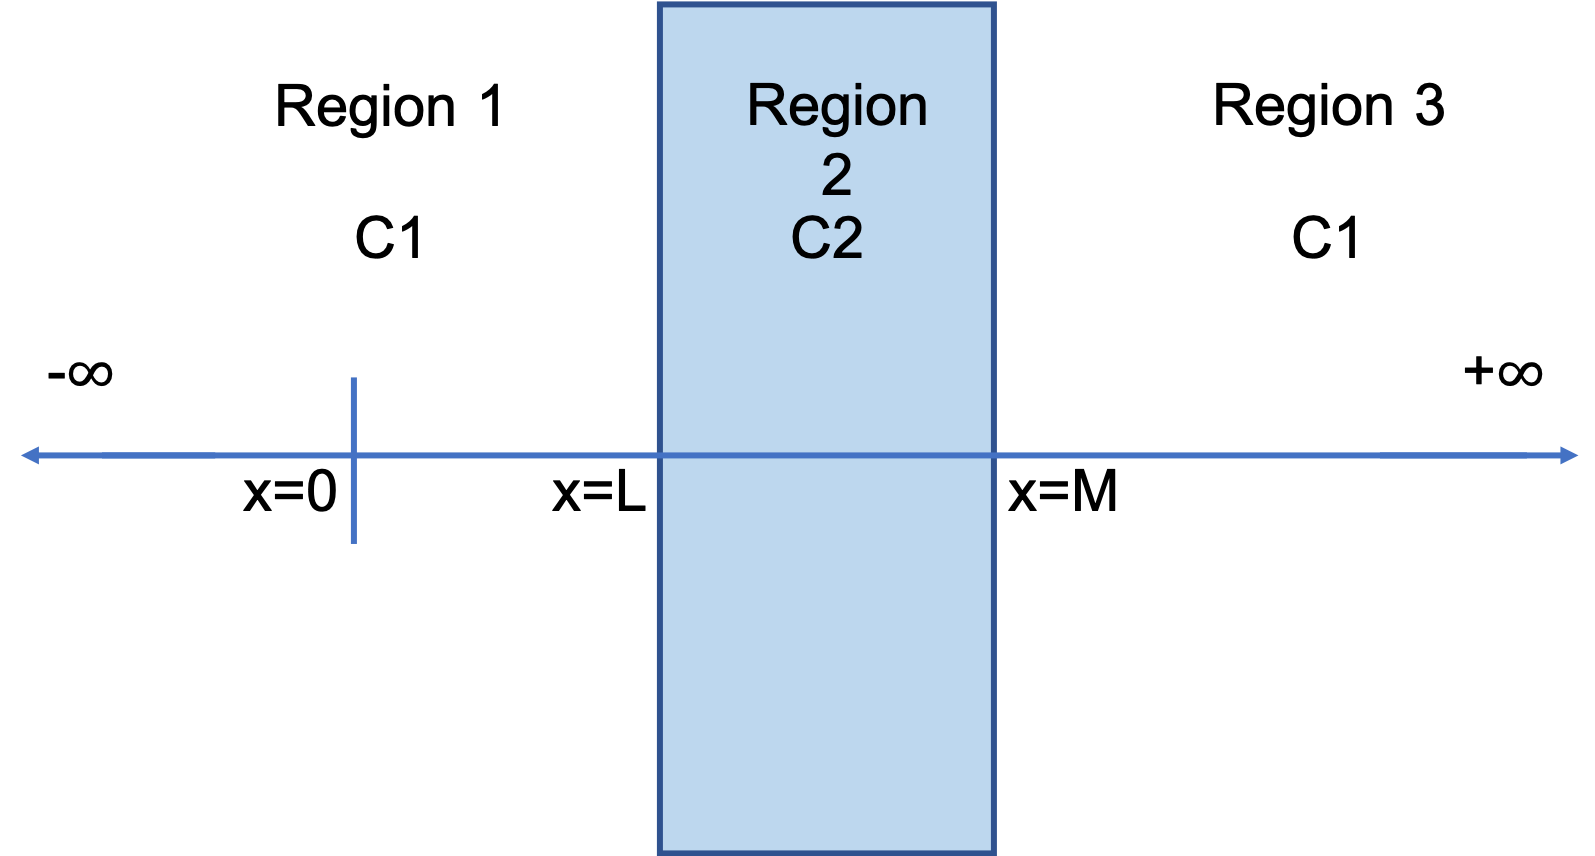
\includegraphics[width=\columnwidth]{regions}
\caption{The simplest generalizable case for propagating a wave through material boundaries involves a single slab (Region 2) of material with a speed coefficient that differs from its surroundings (Region 1 and Region 3, which are semi-infinite).}
\label{fig:regions}
\end{figure}

This problem consists of three distinct regions (See Fig. \ref{fig:regions}). In the first region, a pulse is beginning to propagate from the left at a speed $c_1$. At the right is a material which may have a different speed constant $c_2$, resulting in a reflected wave back into Region 1 and a transmitted wave into Region 2, which initially contains no waves. The transmitted wave from Region 1 travels through Region 2 with a change in velocity and amplitude, then into Region 3, resulting in additional reflected and transmitted waves.

For the purposes of this paper, a wave pulse will be defined with a finite duration and a simple offset-sine-wave form such that the wave intensity increases smoothly from zero up to twice the amplitude, then back down to zero.

%This problem could be modeled using Heaviside step functions at the material boundaries, making $c = \sqrt{\frac{E}{\rho}} = f(x)$. The addition of a variable coefficient poses challenges to solving the full wave equation. An attempt is made to model using three instances of the wave equation. If we are interested in how a stress wave is attenuated over a material ``gap,'' we can focus on how the stress wave hits the material boundary, which can kick off a wave into the next material. 

%Thus, Region 1 may be modeled with a Dirichlet boundary condition on the left-hand side, where the pulse is beginning to move from. On the right hand side is a Robin boundary condition. The solution to the wave equation with these boundary conditions may be obtained using integral transform methods.One result is an explicit equation for $u(L_1,t)$, the equation for wave amplitude at the RHS of Region 1.

%We may use this equation as the input to Region 2; in other words, we set the LHS of Region 2 as a Dirichlet boundary condition with amplitude specified by $u_1(L_1,t)$



%\begin{equation}
%\frac{\partial^2 u}{\partial x^2} = \frac{1}{c^2}\frac{\partial^2 u}{\partial t^2}
%\end{equation}
%
%Where $u = f(x,t)$, i.e., the solution to the wave equation. In this paper, $u(x,t)$ and $u$ will be used interchangeably.
%
%For Region 1, the wave equation is solved  subject to the following initial and boundary conditions:
%
%\begin{equation}
%u(x,0) = \sin(A\pi x) - sin(A\pi x)H(A-x)
%\end{equation}
%
%Where $H$ is the Heaviside function, implying that the initial condition is a pulse of width A, with the value of $u(x,0)$ equal to zero everywhere else.
%
%\begin{equation}
%\frac{\partial u}{\partial t} = 0
%\end{equation}
%
%\begin{equation}
%u(0,t) = 0
%\end{equation}
%
%\begin{equation}
%k_1\frac{\partial u(L_1,t}{\partial x} + h_1 u(x,t) =0
%\end{equation}
%
%The solution corresponds with that found in VIII.3.5.1 by Soloviev. The general solution is:
%
%\begin{multline}
%\sum _{n=1} ^\infty \frac{\sin\lambda_nx}{\frac{L}{2} - \frac{\sin 2 \lambda_n L_1}{4\lambda_n}} \Bigg(\int_0^{L_1} u_0(x)\sin(\lambda_nx)dx \cos(\lambda_nct) \\
% + \frac{\int_0^{L_1}u_1(x)\sin(\lambda_nx)dx}{\lambda_n c}\sin(\lambda_nct)\Bigg)
%\end{multline}
%
%The Sturm-Liouville problem associated with the multi-material wave equation is difficult to solve, 

\subsection{Wave pulse equation}
A wave pulse may be modeled by a modification of the d`Alembert wave  solution as follows:

\begin{equation}
\Big(H(x_n - c_nt) - H(x_n + \lambda_n -c_nt)\Big) u_n(\lambda_n,c_n,x_n,P,x,t)%\Big(\frac{2\pi}{\lambda}(x - (x_n+P) - c_n t)\Big)
\end{equation}

By applying a moving filter function, we are able to isolate a part of the wave form, bounded between $x_n$ and $x_n  +P$, where length of the pulse is denoted $P$, and with $x_n$ as the location of the left-hand endpoint of the pulse function.

The function $u_n$ can actually be any function, but for the implementation in this paper it will take the form:

\begin{equation}
u_n = A_n + A_n \cos\Big(\frac{2\pi}{\lambda_n}(x - \frac{\lambda_n}{2} -x_n - c_n t) \Big)
\end{equation}

\noindent where $A_n$ is the amplitude of the pulse, $\lambda_n$ is the wavelength, $c_n$ is the wave velocity, and $x_n$ is the location of the left-hand-side endpoint of the wave pulse.

\subsection{Material boundary conditions}
Let an incident wave $u_i$ traveling from left to right towards a material boundary at location $x=L$ has amplitude $A$, wavelength $\lambda$, and speed $c_1$. At the $x=L$ boundary, the material properties change immediately to new wave speed $c_2$.

For continuity of the wave form, the following conditions must apply:

\begin{equation}
u_i(L,t) +u_r(L,t) = u_t(L,t)
\end{equation}

\begin{equation}
 \frac{\partial}{\partial x}   u_i(L,t) +  \frac{\partial}{\partial x} u_r(L,t) =  \frac{\partial}{\partial x} u_t(L,t)
\end{equation}

From these conditions can be derived the necessary change in amplitude and effective wavelength that occurs between the incident, reflected, and transmitted waves. For a pulse of amplitude $A$ and wavelength $\lambda_A$, moving from material with speed $c_1$ to material with speed $c_2$ we obtain the following relations:

\begin{equation}
B = A\frac{c_2-c_1}{c_2+c_1}
\end{equation}

\begin{equation}
C = A\frac{2c_2}{c_2+c_1}
\end{equation}

$B$ is the amplitude associated with the reflected wave, and $C$ is the amplitude associated with the transmitted wave. 

\begin{equation}
\lambda_C = \lambda_A \frac{c2}{c_1}
\end{equation}

Note that the reflected pulse has the same speed (opposite-sign velocity) of the incident pulse, and the same wavelength as well.

The concept of ``boundary conditions'' can now be applied to solve for the starting positions of the reflected and transmitted waves. The calculated position is such that the incident, reflected, and transmitted pulses all meet the material boundary at the same time.

\begin{figure}
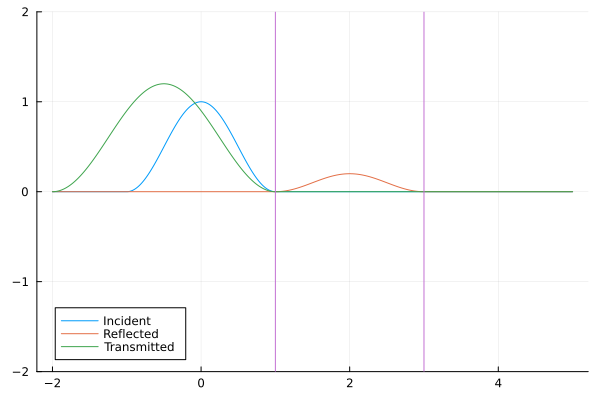
\includegraphics[width=\columnwidth]{Thing6}
\caption{The incident pulse meets the wall at $x=2$ simultaneously with the reflected pulse and transmitted  pulse. All waves are summed only in the regions in which they apply, so at this time frame the reflected and transmitted waves are ``virtual,'' and not included in the wave intensity calculation where presently located. }
\label{fig:pulse-timing}
\end{figure}

\subsection{Implementation of wave equations}
A pulse function may be initialized with the following parameters:

\begin{itemize}
\item Amplitude $A$
\item Wavelength $\lambda$
\item Starting Position $x1$, $x2$
\item Velocity $c$
\end{itemize}

We therefore can define a \texttt{Pulse} object that makes these parameters conveniently available and extensible for many pulse functions. The following algorithm generates pulse functions such that each Region is assigned pulse functions representing every incident, reflected, and transmitted pulse. Mathematically, pulse amplitudes will decay below a threshold after a certain number of transmission/reflection events. This is easily handled with a  \texttt{while} loop. See Algorithm \ref{alg:main}.

\begin{algorithm}
\caption{Generation of Pulse Functions}
\label{alg:main}
\begin{algorithmic}[1]
\State Initialize N Regions $R_1$: $R_n$ with speed of sound $c_1$ to $c_n$
\State Initialize pulse contained in Region 1 with speed $c_1$ moving toward Region 2 \rightarrow Incident
\State Calculate reflected pulse back into Region 1 \rightarrow L1
\State Calculate transmitted pulse into Region 2 \rightarrow  R2
\While{$A> threshold$} 

    \State L2 $=$ \texttt{Reflect}(R2)
    \State  R3 $=$ \texttt{Transmit}(22)
    
    \State R2 $=$ \texttt{Reflect}(L2)
    \State  L1 $=$ \texttt{Transmit}(L2)

\EndWhile
\For{pulse in  pulseList}
	\texttt{GenerateFunction}(pulse)
\EndFor


\Return{List of Pulse Functions per region}

\end{algorithmic}
\end{algorithm}

\begin{algorithm}
\caption{Reflect}
\label{alg:reflect}
\begin{algorithmic}[1]
\State Inputs: \texttt{Pulse} object with $A$, $\lambda$, $c$, $x_0$, 
\State Boundary Location $L$ and $c_L$ on other side of boundary
\State $A_R$ = \texttt{Pulse}.Amplitude*(c2-c1)/(c2+c1)
\State $x_R$ = L + L -\texttt{Pulse}.position - \texttt{Pulse}.wavelength
\State ReflectedPulse = \texttt{PulseObject}($A_R$,\texttt{Pulse}.wavelength,$x_R$, -\texttt{Pulse}.speed)

\Return{ReflectedPulse}

\end{algorithmic}
\end{algorithm}

\begin{algorithm}
\caption{Transmit}
\label{alg:transmit}
\begin{algorithmic}[1]
\State Inputs: \texttt{Pulse} object with $A$, $\lambda$, $c$, $x_0$, 
\State Boundary Location $L$ and $c_L$ on other side of boundary
\State $A_T$ = \texttt{Pulse}.Amplitude*(2*c2)/(c2+c1)
\State $\lambda_T$ = c2/c1*\texttt{Pulse}.wavelength
\State $x_T$ = -c2/c1 * (-\texttt{Pulse}.position+L+A.wavelength) + L + $\lambda_T$
\State TransmittedPulse = \texttt{PulseObject}($A_T$, $\lambda_T$, $x_T$, \texttt{Pulse}.speed *$c_L$)

\Return{TransmittedPulse}

\end{algorithmic}
\end{algorithm}

\newpage
\section*{Results}
Four initial cases are completely simulated and results are available at \url{https://github.com/tekajuna/pulse-thru-wall}. 

For each case, $c_1 = 2.0$, $c_2 = 8.0$, the wall spans from $x=2.0$ to $x=3.0$, and one pulse is located with the left endpoint at the origin with an amplitude of $0.5$. A second pulse is also initialized as follows:

\begin{enumerate}
\item Second pulse is located at $x=-2$ with amplitude $0.5$ (Pulses separated by one wavelength)
\item Second pulse is located at $x=-1$ with amplitude $0.5$ (Two pulses appear as a single sine wave with two full periods)
\item Second pulse is located at $x=-0.5$ with amplitude $0.5$ (Sine wave with a flattened top due to partial interference)
\item Second pulse is located at $x=-1$ with amplitude $-0.5$ (Second pulse is reflected across x-axis, resulting in the appearance of a full-period sine wave with amplitude of 1 and no vertical offset)

\end{enumerate} 


Two parameter variations studies were performed. In the first, the starting position of one of two identical pulses is varied. The stationary pulse is located at the origin, as in the Cases 1 through 4. The varied-position pulse is located at positions between $x=-1$ and $x=1$. At $x=0$, the two pulses constructively interfere, resulting in a single pulse with double amplitude. For each starting position of the second pulse, the maximum wave intensity value in Region 2 is plotted.

\begin{figure}
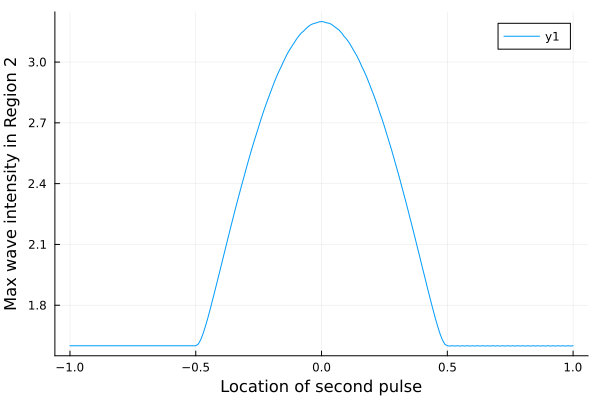
\includegraphics[width=\columnwidth]{PulseSpacing}
\caption{Starting location of one pulse was varied with respect to the starting location of the other, effectively varying the relative time-of-arrival of two pulses to the first material boundary. Both pulses have positive amplitude, resulting in varying degrees of constructive interference. The peak wave intensity within Region 2  is maximized when the pulses totally interfere constructively, resulting in a wave amplitude over three times that of the individual pulses }
\label{fig:study1}
\end{figure}

The second parameter variation study is similar to the first, but the second pulse has negative amplitude, resulting in perfectly destructive interference when $x=0$. Peak Region 2 wave intensity is found when $x=\pm 0.5$

\begin{figure}
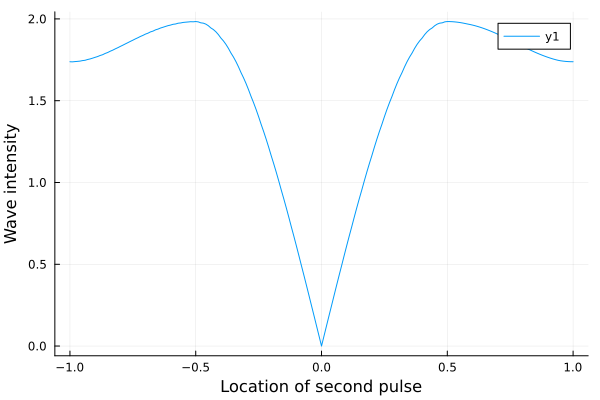
\includegraphics[width=\columnwidth]{PulseSpacingReverse}
\caption{The second pulse in this case has a negative amplitude. Starting location of this pulse was varied with respect to the starting location of the other. Varying degrees of destructive interference is observed. The peak wave intensity within Region 2  is maximized when there is a certain amount of offset between the negative and positive pulses.}
\label{fig:study2}
\end{figure}





\begin{comment}
\section*{Body Sections Go Here}
The text should be organized into logical parts or sections. THe purpose of the paper, or the author's aim, should be stated at the beginning so that the reader will have a clear concep tof the paper's objective. This should be followed by a description of the problem, the means of solution, and any other information necessary to properly qualify the results presented and the conclusions. Finally, the results should be presented in an orderly form, followed by the author's conclusions. 

To make a reference to a particular figure, do this: Figure \ref{fig:sample}, followed by 
\begin{figure}
    % \includegraphics{"sample.png"}
    \caption{Empty figure sample.}
    \label{fig:sample}
\end{figure}
This assumes the image file is found in the same directory as this .tex file.

To make a reference to a document in your bibliography, do this: in \cite{textbook}, ....
This requires you to create a .bib file, of which an example should come with this document.

\end{comment}


\section*{Conclusions}
A method for analyzing wave pulse behavior across material boundaries has been developed. The method developed involves a single slab of material sandwiched between semi-infinite regions of the same material property $c_1$, but adding additional finite regions is easily accomplished. Present development includes one particular type of wave pulse, but the concepts are easily extensible to other pulse functions, such as semi-infinite, sawtooth, Gaussian, and Lorentzian pulse/wave variants. 

Further development should aid in the interpretation of the pulse intensity, which in this paper may be best interpreted as the transverse amplitude of a wave. In other cases it is desirable to understand pressure or stress intensities associated with longitudinal waves propagating through fluid or solid materials. 




%\section*{Acknowledgements}
%Thanks to Dr. Soloviev for 

% The bibliography is automatically generated from template.bib. Rename template.bib to match this file's name, if you change it. This will require an installation of Biber, which you should not install by hand; you run Latex on this document, then Biber on the shared name (e.g. "template"), then Latex again.
% The names you give in the template.bib file become the names you can cite in this document.
\printbibliography

\onecolumn
\section*{Appendix}

\subsection*{Julia code for pulse analysis and plotting}
%Young's Modulus per density: 10$^6$ m$^2$$/$s$^2$
%\begin{itemize}
%\item Aluminum: 26
%\item Silicon: 79
%\item Steel: 25
%\item Copper: 13
%\item Zinc: 15
%\item Tungsten: 21
%\item Sapphire: 101
%\item Beryllium: 155
% \item Diamond: 347
%\end{itemize}
\begin{verbatim}
using Plots

struct Pulse #Characteristics of a pulse
    amplitude
    wavelength
    position # Position of the LHS of the pulse
    speed
end

function filter(A::Pulse, x1,x2,x,c,t,f)
    if x < x1+c*t # pulse is defined only on interval x1 to x2
        return 0
    elseif x > x2 + c*t
        return 0
    else
        return f(x,t) # Pulse can have any functional definition between the endpoints
    end
end

function cosWaveFunction(A,lambda,c,x1)
    function wave(x,t)
        return A + A*cos(2*pi/lambda*(x - 0.5*lambda -x1 - c*t) ) #centers the pulse within [x1, x2]
    end
    return wave
end

function generatePulse(A::Pulse)
    # TODO: Specify location and direction of the pulse
    function pulse(x,t)
        x1 = A.position # Pulse is located left of the origin
        x2 = A.position + A.wavelength       # RHS of the pulse is at the origin
        f = cosWaveFunction(A.amplitude,A.wavelength,A.speed,A.position)
        return filter(A,x1,x2,x,A.speed,t,f)

    end
    return pulse
end

function Reflect(A::Pulse, L,cL)
    c1 = abs(A.speed)     # Characteristic Speed of the Incidient wave
    c2 = abs(cL) # Characteristic speed on the OTHER side of "L"
    ampR = A.amplitude*(c2-c1)/(c2+c1) # Calculate amplitude of the reflected wave (absolute value)
    lamR = A.wavelength # Reflected wave has same wavel. as incident
    posR = L + L -A.position - A.wavelength   #Reflected wave is positioned 
    Rpulse = Pulse(ampR,lamR,posR,-A.speed)
    return Rpulse
end

function Transmit(A::Pulse,L,cL)
    c1 = abs(A.speed) # Velocity of the incident wave
    c2 = abs(cL)      # Speed of target material
    ampT = A.amplitude * 2*c2/(c2+c1)
    lamT = c2 *A.wavelength/c1
    posT = -c2/c1*(-A.position+L+A.wavelength) +L +lamT
    Tpulse = Pulse(ampT,lamT,posT,sign(A.speed)*cL)
    return Tpulse
end

function calculatePulses(inc,c1,c2, L, M)
    Reg1 =[]
    Reg2 =[]
    Reg3 =[]
    # R Right-moving 
    # L Left-moving
    # Number indicates region
    R1 = inc            # Incident Wave
    push!(Reg1,R1)
    L1 = Reflect(inc,L,c2)   # Reflects toward negative infinity
    push!(Reg1,L1)
    R2 = Transmit(inc,L,c2)  # Transmits toward M
    push!(Reg2,R2)
    # L2 = Reflect(R2)    # Internal Reflection
    # R3 = Transmit(R2)   # Transmits toward infinity
    # L1 = Transmit(L2)   # Transmits to negative infinity
    # R2 = Reflect(L2)    # internal Reflection
    # L2 = Reflect(R2)
    # R3 = Transmit(L2)
    # generates:
    # L1, R2
    # L2, R3
    # L1. R2
    # L2, R3

    while abs(R2.amplitude) > 1e-3 #Calculate reflections until amplitude goes below threshold
        L2 = Reflect(R2,M,c1)    # Internal Reflection
        push!(Reg2,L2)
        R3 = Transmit(R2,M,c1)   # Transmits toward infinity
        push!(Reg3,R3)
        L1 = Transmit(L2,L,c1)   # Transmits to negative infinity
        push!(Reg1,L1)
        R2 = Reflect(L2,L,c1)
        push!(Reg2,R2)
    end
    # println(length(Reg1))
    # println(length(Reg2))
    # println(length(Reg3))
    #Transform pulse objects to functions
    for i = 1:length(Reg1)
        Reg1[i] = generatePulse(Reg1[i])
    end
    for i = 1:length(Reg2)
        Reg2[i] = generatePulse(Reg2[i])
    end
    for i = 1:length(Reg3)
        Reg3[i] = generatePulse(Reg3[i])
    end


    return Reg1, Reg2, Reg3
end

function testPulseGeneration()
    c1 = 8.0
    c2 = 2.0
    L  = 1.0
    M  = 3.0
    N  = 5.0
    initialPulse = Pulse(1.0,1,0,c1)
    R1,R2,R3 = calculatePulses(initialPulse,c1,c2, L, M)
    println("Neat")
end

function analyze()


end

function testRegions()
    c1 = 2.0
    c2 = 8.0
    L  = 2.0
    M  = 3.0
    N  = 5.0
    initialPulse = Pulse(0.5,1,0,c1)
    R1,R2,R3 = calculatePulses(initialPulse,c1,c2, L, M)
    additionalPulse=Pulse(-0.5,1,-0.5,c1)
    R1b,R2b,R3b = calculatePulses(additionalPulse,c1,c2, L, M)
    

    # A = generatePulse(initialPulse)
    # push!(R1,A)
    # B = generatePulse(Reflect(initialPulse,L,c2))
    # C = generatePulse(Transmit(initialPulse,L,c2))
    # push!(R1,B)
    # push!(R2,C)
    tvec = 0:0.01:5.0
    x1 = 0.0:0.01:L
    x2 = L:0.01:M
    x3 = M:0.01:N
    for i = 1:length(tvec)
        t = tvec[i]
        # plot(x,A.(x,t),label="I")
        # plot!(x,B.(x ,t),label="R1")
        # plot!(x,C.(x,t),label="T1")
        # u1 = R1[1].(x1,t) + R1[2].(x1,t)
        u1 = sum([R1[i].(x1,t) for i in 1:length(R1)])+sum([R1b[i].(x1,t) for i in 1:length(R1b)])
        u2 = sum([R2[i].(x2,t) for i in 1:length(R2)])+sum([R2b[i].(x2,t) for i in 1:length(R2b)])
        u3 = sum([R3[i].(x3,t) for i in 1:length(R3)])+sum([R3b[i].(x3,t) for i in 1:length(R3b)])
        # plot(x1,A.(x1,t)+B.(x1,t))
        plot(x1,u1)
        plot!(x2,u2)
        plot!(x3,u3)
        # plot!(x2,C.(x2,t))
        # plot!(x3,zeros(length(x3)))
        vline!([L,M])
        ylims!((-2,2))
        if i <10
            savefig("nice4/Thing00"*string(i)*".png")
        elseif i < 100
            savefig("nice4/Thing0"*string(i)*".png")
        else
            savefig("nice4/Thing"*string(i)*".png")
        end

    end


end

function varyPulseSpacing()
    c1 = 2.0
    c2 = 8.0
    L  = 2.0
    M  = 3.0
    N  = 5.0
    initialPulse = Pulse(-0.5,1,0,c1)
    R1,R2,R3 = calculatePulses(initialPulse,c1,c2, L, M)


    xAddl = -1:0.1:1 # Vary Second Pulse location; otherwise pulses are identical
    maxR2 = []
  
    for k = 1:length(xAddl)
        additionalPulse=Pulse(0.5,1,xAddl[k],c1)
        R1b,R2b,R3b = calculatePulses(additionalPulse,c1,c2, L, M)
        tvec = 0:0.01:5.0
        x1 = 0.0:0.01:L
        x2 = L:0.01:M
        x3 = M:0.01:N
        maxtemp=0 # Reset max pulse intensity for the current initial pulse spacing
        for i = 1:length(tvec)
            t = tvec[i]
            # plot(x,A.(x,t),label="I")
            # plot!(x,B.(x ,t),label="R1")
            # plot!(x,C.(x,t),label="T1")
            # u1 = R1[1].(x1,t) + R1[2].(x1,t)
            u1 = sum([R1[i].(x1,t) for i in 1:length(R1)])+sum([R1b[i].(x1,t) for i in 1:length(R1b)])
            u2 = sum([R2[i].(x2,t) for i in 1:length(R2)])+sum([R2b[i].(x2,t) for i in 1:length(R2b)])
            u3 = sum([R3[i].(x3,t) for i in 1:length(R3)])+sum([R3b[i].(x3,t) for i in 1:length(R3b)])
            if maximum(abs.(u2)) > maxtemp
                maxtemp = maximum(abs.(u2))
            end

        end
        push!(maxR2,maxtemp)
    end
    plot(xAddl,maxR2)
    xlabel("Pulse Spacing")
    ylabel("Max Wave Intensity")
    savefig("figs/PulseSpacingReverse.png")

end




function testdalambert()
    amp = 0.5
    wavel=2
    c1 = 2.0
    c2 = 3.0
    L = 1.0 # Position of the first wall, transitioning from c1 to c2
    M = 3.0
    N = 5.0
    initialPulse = Pulse(amp,wavel,-wavel,c1)
    A = generatePulse(initialPulse) # Generate Incident pulse # Amplitude, wavelength, LHS location
    Rpulse = Reflect(initialPulse,L,c2)
    B = generatePulse(Rpulse)
    Tpulse = Transmit(initialPulse,L,c2)
    C = generatePulse(Tpulse)
    D = generatePulse(Reflect(Tpulse,M,c1))
    E = generatePulse(Transmit(Tpulse,M,c1))
    # t = 0 
    tvec = 0.0:0.1:8.0

    # R1 0 to L
    # R2 L to M
    # R3 M to N 

    x = -2.0:0.01:N

    for i in range(1,length(tvec);step=1)
        t = tvec[i]
        plot(x,A.(x,t),label="Incident")
        plot!(x,B.(x ,t),label="Reflected")
        plot!(x,C.(x,t),label="Transmitted")
        # plot!(x,D.(x,t),label="R2")
        # plot!(x,E.(x,t),label="T2")
        vline!([L,M],label=nothing)
        ylims!((-2,2))
        plot!(legend=:bottomleft)
        
        # legend
        savefig("TP/Thing"*string(i)*".png")

    end


end
if abspath(PROGRAM_FILE) ==@__FILE__
    # testdalambert()
    # testRegions()
    # testPulseGeneration()
    varyPulseSpacing()
end
\end{verbatim}

\end{document}
